\documentclass[]{article}
\usepackage[utf8]{inputenc}
\usepackage[pdftex]{graphicx} % for includegraphics
\usepackage[bf,font={small,sl}]{caption} % for pretty captions
\usepackage{natbib} % for the bibliography

\title{\texttt{moveHMM}\\ An R package for animal movement modelling}
\author{Michelot T., Langrock R., Patterson T., and Rexstad E.}

\begin{document}
\maketitle

\section*{Introduction}
Animal movement data is growing rapidly, due to the substantial improvement of telemetry technologies. As a result, statistical methods used to analyse this data are brought to their computational limit.

Novel models have been developed in the last decade to reduce the computational cost of statistical inference in movement ecology. In particular, hidden Markov models are increasingly popular in this field, due to their flexibility, and to the efficient algorithms that they offer, see \cite{patterson2009} and \cite{langrock2012}.\\

\texttt{moveHMM} is an R package which implements hidden Markov models (HMMs) for animal movement. A special attention was paid to performance, and the fitting algorithm is implemented in C++ to make it significantly faster.

The goal of this vignette is to give a global overview of the possibilities offered by the package, and to demonstrate its use on a detailed example.

\section{Package features}
In this section, we describe different features included in \texttt{moveHMM}. We describe the global structure of the package, and then describe in more detail the main functions required to fit a HMM to movement data. In particular, we introduce the different options that the functions offer, and explain how the functions' arguments should be chosen.

\subsection{Structure}
The package is articulated around two S3 classes : \texttt{moveData} and \texttt{moveHMM}. The first one is a data frame of the data, essentially gathering time series of the movement metrics of interest, namely the step lengths and turning angles, as well as the covariate values. A \texttt{moveHMM} object is a fitted model, which stores in particular the values of the MLE of the parameters.\\

In order to create a \texttt{moveData} object, the function \texttt{prepData} is called on the tracking data (track points coordinates). Then, the function \texttt{fitHMM} is called on the \texttt{moveData}, and returns a \texttt{moveHMM}.

Both classes can be used through their methods, e.g. \texttt{plot.moveData}, \texttt{decode.moveHMM}, \texttt{AIC.moveHMM}... All the functions are described in more detail in Section \ref{main_functions}, and their use is explained on an example in Section \ref{application}.\\

Figure \ref{struct} illustrates the links between the main components of the package.

\begin{figure}[h]
	\centering
	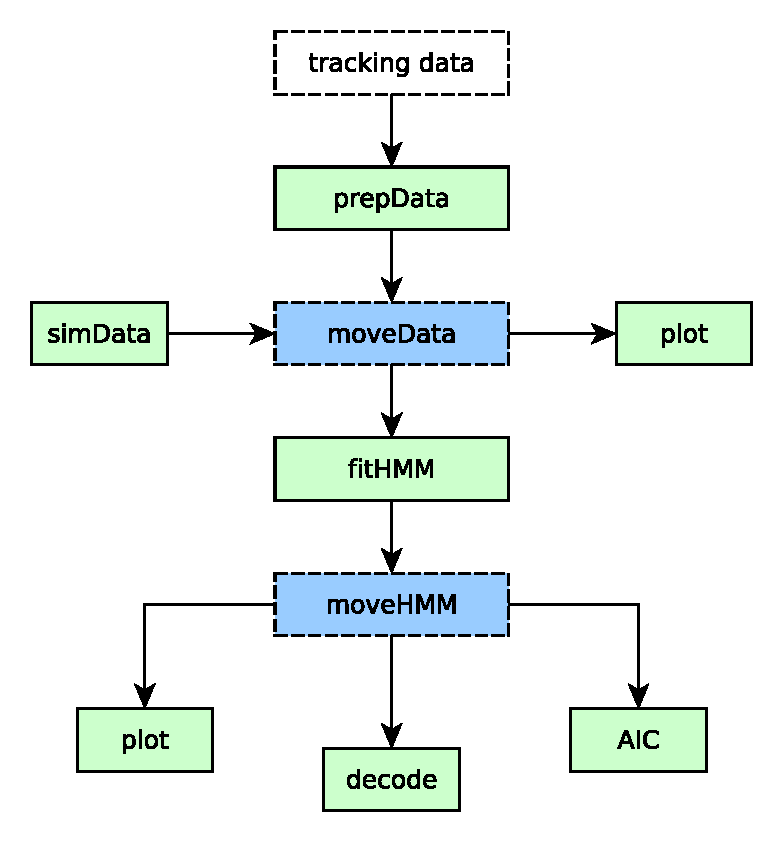
\includegraphics[width=0.5\textwidth]{pictures/struct}
	\caption{Structure of the main components of the package. The blue boxes are S3 classes, and the green boxes are functions. The arrows indicate input and output of data.}
	\label{struct}
\end{figure}


\subsection{Main functions} \label{main_functions}
We list the main user functions, and discuss the options they include, e.g.
\begin{itemize}
	\item step and angle distributions:
	\item zero-inflation for the step distribution;
	\item covariates for the transition probabilities;
	\item step-length modelling only;
	\item stationary model;
	\item angle mean estimation or not;
	\item ...
\end{itemize}
We can also mention and justify the default values of the options.

\subsubsection{prepData}

\subsubsection{fitHMM}

\subsubsection{Classes methods}

\subsubsection{simData}

\section{Application} \label{application}
We take the user through a detailed example. I think that we will include a (relatively small) real data set in \texttt{data/}, which will serve in this example.

\subsection{Movement data}
We describe the format of the data that the user needs to input :
\begin{itemize}
	\item R data frame;
	\item regular time intervals;
	\item mandatory column names : "ID", "x", "y", ...;
	\item additional columns are considered as covariates;
	\item warn the user about missing covariate values;
	\item warn the user about outliers.
\end{itemize}

We explain how to use the function \texttt{prepData} to transform the tracking data into movement data.

We explain how to use \texttt{plot.moveData}, which graphical options are available, and we display the output.

\subsection{Fitting the model}
We go through all the options of \texttt{fitHMM}, and demonstrate its use on the real data example.

Here we can warn the user about the choice of the initial values.

\subsection{Using the model}
We need to mention :
\begin{itemize}
	\item Plotting : describe the function \texttt{plot.moveHMM} and the graphical options, and display all the plots;
	\item Decoding : describe the decoding functions, such as \texttt{viterbi}, \texttt{stateProbs}, and \texttt{pseudoRes}, and apply them to the data;
	\item Assessing : we don't really have the functions yet, but we will need to explain how to obtain confidence intervals, and how to plot them. We might want to mention the simulation function as an assessing tool.
\end{itemize}


\begin{thebibliography}{}

\bibitem[\protect\citeauthoryear{Langrock}{2012}]{langrock2012}
\textsc{Langrock R., King R., Matthiopoulos J., Thomas L., Fortin D., Morales J.M.} (2012),
``Flexible and practical modeling of animal telemetry data: hidden Markov models and extensions''
\textit{Ecology}, 93 (11), 2336-2342.

\bibitem[\protect\citeauthoryear{Patterson}{2009}]{patterson2009}
\textsc{Patterson T.A., Basson M., Bravington M.V., Gunn J.S.} (2012),
``Classifying movement behaviour in relation to environmental conditions using hidden Markov models''
\textit{Journal of Animal Ecology}, 78 (6), 1113-1123.

\end{thebibliography}

\end{document}